%%%%%%%%%%%%%%%%%%%%%%%%%%%%%%%%%%%
% PART II: Experiment definition module
%%%%%%%%%%%%%%%%%%%%%%%%%%%%%%%%%%%

\part{The Abstract Experiment Definition Language -- AEDL}

\chapter{Getting started}

Here the general concept of the AEDL is described and illustrated by an example. In addition, a short introduction to the syntax of the AEDL is given.

\section{General concept of the experiment simulation}

The goal of AEDL is to describe a large number of complex and very 
different experiments by a limited number of parameters. It allows a
representation of very different setups within one data structure, and thus implements universal rate and $\chi^2$ computation methods. For experiment simulations, a new piece of code is usually written and compiled
for each different experiment. In many cases, even parameter changes, such as
the number of bins, requires the recompilation of the source code. 
However, such a technique soon reaches its limits when the simulated experiments are rather complex, or more than one type of experiment is studied simultaneously. Furthermore, it is very difficult to verify the correctness of the obtained results, since every time a new piece of code is added to 
deal with a new experiment type, new errors will be introduced.

Thus, a general and flexible experiment description language is needed.  
The description of a neutrino experiment can be split into three parts: Source, oscillation, and detection. The neutrino sources within \GLOBES\ 
are assumed to be stationary point sources, where each experiment has only 
one source. This restricts the classes of neutrino sources which can be studied with \GLOBES :
\begin{itemize}
\item
 Experiments using many point-like sources can only be approximated. One example are reactor experiments using many distant reactor blocks.
\item
 Geometrical effects of a source distribution, such as in the sun or the atmosphere, can not be described.
\item
 Sources with a physically significant time dependencies  can not be studied, such as  supernov\ae. It is, however, possible
to study beams with bunch structure, since the time dependence of the
neutrino source is physically only important to suppress backgrounds. 
\end{itemize}

The description of the neutrino oscillation physics is, at least numerically, relatively simple. We use the {\em evolution operator method} to compute the neutrino oscillation probabilities and divide the matter density profile into layers with constant matter densities. For each of these layers, the Hamiltonian in matter is diagonalized in order to propagate the neutrino transition amplitudes. Finally, the transition probability is obtained by the absolute square of the total neutrino transition amplitudes. Depending on the precision of the studied experiment, this approach turns out to be precise enough in Earth matter even for a small number matter density steps. Since we allow an uncertainty of the matter density profile, it is, in fact, in most cases sufficient to consider only one density step with the average matter density together with a matter density uncertainty~\cite{Ohlsson:2003ip}. Note that this approach may not be applicable to quickly varying extraterrestrial matter density profiles.

While it is comparatively simple to define a general neutrino source 
and to compute the oscillation physics, the general properties of a detector simulation are much more complicated. The basic assumption in building an abstract detector description is \emph{linearity}, \ie , that two neutrino events do not interfere with each other. Furthermore it is assumed that all information on the oscillation physics 
is given by the \emph{reconstructed} flavor and energy of a 
neutrino event. The term ``reconstructed'' implies that the well-defined energy of the incident neutrino, which can not be directly observed, translates via secondary particles and the detection properties into a distribution of possible energy values. This process is illustrated in \figu{distro} for the energy variable. 
%
\begin{figure}[ht]
\begin{center}
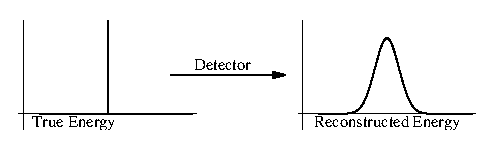
\includegraphics[width=0.6\textwidth]{mapping}
\end{center}
\caption{\label{fig:distro} A detector maps a true parameter value onto
a distribution of reconstructed parameter values. This is illustrated here for there energy.}
\end{figure}
% 
The same, in principle, applies to the nature of the neutrino flavor. However, in this case only discrete values are applicable. Note that the reconstructed neutrino energy and the neutrino flavor are the only observables in \GLOBES .

This picture can also be formulated in a more mathematical way. Let us define $x$ as the true parameter value and $x'$ as the reconstructed parameter value. Similarly, $f(x)$ is the distribution of true parameters values and $p(x')$ is the distribution of reconstructed parameter values. Then the detector function  $D(x,x')$, which describes the mapping performed by the detector, is given by
\begin{eqnarray}
\label{equ:mapping}
p(x')&=&\int dx\, f(x)\cdot D(x,x')\,.
\end{eqnarray}
Obviously \equ{mapping} only describes the detector properly
if the linearity condition is fulfilled. Within this model, a detector
is completely specified by a set of $D(E,E')$ for the energy variable $E$,
and a set $D(F,F')$ for the flavor variable $F$. In general, $D(E,E')$ also depends on the true flavor $F$, as well as $D(F,F')$ depends on the true energy $E$. These sets of mapping functions usually are obtained from a 
full detector simulation and can be obtained by using as input 
distribution $f(x)$ a delta distribution $\delta(x-x_0)$.

In order to implement a experiment definition including various
sources of systematical errors, we use several abstraction levels. 
The first level is the so-called ``channel'', which is the link between 
the oscillation physics and the detection properties for a specfific oscillation pattern. A channel specifies the mapping of a specific neutrino flavor produced by the source onto a reconstructed neutrino flavor.
For example, a muon neutrino oscillates into an electron neutrino and subsequently interacts via quasi-elastic charged current scattering. The measured energy and direction of
the secondary electron in the detector then allows to reconstruct the neutrino energy. The connection from the source flux of the muon neutrino, via the  probability to appear as a electron neutrino, to its detection properties (such as cross sections and energy smearing) is encapsulated into the channel.

The channels are the building blocks for the so-called ``rules''. In general, a rule consists of one or more ``signal'' and ``background'' oscillation channels, which are normalized with efficiencies. The event numbers from these channels are added {\em before} the $\chi^2$-value is calculated. In addition, each rule implements an {\em independent} systematics, such as signal and background normalization errors. Eventually, each rule gives a $\chi^2$-value, and the total $\chi^2$ is obtained by adding the $\chi^2$'s of all rules. 
 An example for a rule could look like this: We want to detect electron neutrino appearance (``signal''), where the overall efficiency for quasi-elastics electron neutrino events is $0.4$. There is a fraction of $0.01$ of all neutral current events which are mis-identified as quasi-elastic electron neutrino events (``background''). The neutral current fraction is only known within $10\%$ (``background uncertainty'') and there is
an energy scale uncertainty of $100\,\mathrm{MeV}$ (``energy calibration error'').
All this systematics is independent of the other rules.  Thus, a rule connects the event rates to the calculation of a $\chi^2$ which properly includes 
systematical errors. The resulting $\chi^2$ is then the starting point for the
oscillation physics analysis. Note again that
\begin{itemize}
\item
 Within each rule the event numbers are added.
\item
 Within each rule the systematics is treated independently from the other rules.
\item
 For each rule the $\chi^2$ is computed; the $\chi^2$'s from all rules are added.
\end{itemize}

Of course, an abstract experiment definition language can not simulate all possible types of experiments. As we have seen, there are several assumptions for source and detector. However, it turns out that \GLOBES\ can be applied to a large number of experiment types, such as conventional beams, superbeams, neutrino factories, $\beta$-Beams, and reactor experiments.

\section{A simple example for AEDL}

Experiments are in \GLOBES\ defined by the Abstract Experiment Definition Language (AEDL). The experiment definition is written into a text file using the AEDL syntax. Currently, a number of pre-defined experiment definition files are provided with \GLOBES , which have to be modified manually in order to define new experiments. An IDE (Integrated Developement Environment) for AEDL files is currently in preparation. The application software then uses this text file to initialize the experiment, where other secondary files might read for source fluxes, cross sections \etc . In this section, we show the definition of a very simple neutrino factory in AEDL, where we do not go into details. In the next chapter, we will discuss each of the individual steps in detail.

The first line of every experiment definition file has to be
\begin{quote}
{\tt !\%GLoBES}
\end{quote}
in order not to confuse it with some other file format.
%
First, we instruct \GLOBES\ to use the built-in source flux for a neutrino factory
originating from stored $\mu^+$'s. Therefore, we set the {\tt @builtin} variable to $1$. Next, we specify the muon energy to be $50\,\mathrm{GeV}$ by the {\tt @parent\_energy} variable. We assume 
that there will be $5.33\cdot 10^{20}$ useful muon decays per year
and that this luminosity is available for $8$ years, \ie , a total number
of $ 4.264\cdot10^{21}$ muons is stored:
\begin{quote}
{\tt /* beam */}\\
{\tt flux(\#mu\_plus)<\\
\tb  @builtin = 1\\
\tb  @parent\_energy = 50.0\\
\tb  @stored\_muons = 5.33e+20\\
\tb  @time = 8.0\\
>}\\
\end{quote}
Note that we tell \GLOBES\ that we want to refer to this neutrino source later as as {\tt \#mu\_plus}. 
%
Let us now define a very simple detector with a target mass 
of $50\,\mathrm{kt}$ and $20$ energy bins between
$4\,\mathrm{GeV}$ and $50\,\mathrm{GeV}$: 
\begin{quote}
{\tt \$target\_mass = 50}\\
{\tt \$numofbins = 20}\\
{\tt \$emin = 4.0}\\
{\tt \$emax = 50.0}
\end{quote}
Then we specify the file which contains the cross sections we want to 
use:
\begin{quote}
{\tt /* cross section */}\\
{\tt cross(\#CC)<}\\
{\tt \tb @cross\_file = XCC.dat}\\
{\tt >}
\end{quote}
The command {\tt cross} tells the parser that a cross section environment
begins. It has the name {\tt \#CC}, which can later be used to refer 
to this specific environment, and thus to the file {\tt XCC.dat}. Note that each name begins with a leading {\tt \#}.
%
Of course, the baseline and matter profile have to be specified, too:
\begin{quote}
{\tt /* baseline */}\\
{\tt \$baseline = 3000.0}\\
{\tt \$densitytab = \{3.5\}}\\
{\tt \$lengthtab = \{3000.0\}}\\
{\tt \$density\_error = 0.05}
\end{quote}
The curly brackets used for the definition of {\tt \$densitytab} and
{\tt \$lengthtab} refer to a list of numbers. Here, the lists contain only
one element, because we only use one density layer: We initialize a baseline length of $3000 \, \mathrm{km}$ with a constant matter density of $3.5 \, \mathrm{g/cm^3}$ and a matter density uncertainty of $5\%$ ($1 \sigma$ relative error). Note that the elements in {\tt \$lengthtab} have to add up to the baseline length. 
%
As another ingredient, we have to define the energy resolution function:
\begin{quote}
{\tt /* energy resolution */}\\
{\tt energy(\#MINOS)<}\\
{\tt \tb @type = 1}\\
{\tt \tb @sigma\_e = \{0.15,0.0,0.0\}}\\
{\tt >}
\end{quote}
The {\tt energy} command starts the energy environment, which has the name 
{\tt \#MINOS} here. Out of several possibilities, it uses algorithm one,
the simplest and fastest one. The actual energy resolution is specified
by the energy resolution variable, which is a list of three elements. Each 
element is one parameter of the general resolution function as defined in 
\eq~\ref{eq:sigma_e}.
%
Now we have all pieces to be able to define the appearance and the corresponding disappearance channel of a neutrino factory: 
$\nu_e\rightarrow\nu_\mu$  and $\bar\nu_\mu\rightarrow\bar\nu_\mu$ 
($\mu^+$ stored).
\begin{quote}
{\tt /* channels */}\\
{\tt channel(\#appearance)<}\\
{\tt \tb @channel = \#mu\_plus: +: electron: muon: \#CC: \#MINOS}\\
{\tt >}\\
{\tt channel(\#disappearance)<}\\
{\tt \tb @channel = \#mu\_plus: -: muon: muon: \#CC: \#MINOS}\\
{\tt >}
\end{quote}
The first element is the name of the flux, which we have already defined above as defined above. The second element $\pm$ determines whether 
neutrinos or anti-neutrinos are taken from the flux table (two different polarities allowed). The third position defines the initial flavor,
and the forth position the final flavor, followed by the name of the cross
section and energy resolution function as defined before.
%
The last step is to encapsulate the channels into a rule:
\begin{quote}
{\tt /* rules */}\\
{\tt rule(\#rule1)<}\\
{\tt \tb @signal = 0.45 @ \#appearance}\\
{\tt \tb @signalerror = 0.001 : 0.0001}\\
{\tt \tb @background = 1.0e-05 @ \#disappearance}\\
{\tt \tb @backgroundcenter = 1 : 0.0}\\
{\tt \tb @backgrounderror = 0.05 : 0.0001}\\
{\tt \tb @errordim = 0}\\
{\tt \tb @energy\_window = 4.0 : 50.0}\\
{\tt >}
\end{quote}
The {\tt @signal} refers to the ``signal'' in our experiment. We use the
above defined channel named {\tt \#appearance} with an constant overall
efficiency of $0.45$. The signal error variable has two components: 
The first one is the normalization error of the signal, here $0.1\%$. The second 
one refers to the energy calibration error of the signal, which is defined 
in \Sec~\ref{sec:energy}. The background variable
specifies the composition of the beam background. In this (simplified) case, we
use the fraction $1\cdot 10^{-5}$ of the channel named {\tt \#disappearance}, \ie , the muon neutrinos with a mis-identified charge. The background center variable allows to rescale the total background contribution from all background components
simultaneously. It is only useful if there is more than one background component, otherwise it is usually $1$. The background error variable is defined such as the signal error variable, \ie\ we have a $5\%$ background uncertainty and a very small energy calibration error. The ``error dimension variable'' {\tt @errordim} selects how the systematical errors are treated (\cf, \Tab~\ref{tab:error_dim}). 

The here defined experiment represents a first simplified version of a neutrino factory experiment. It still lacks the correct energy dependence of the efficiencies, the antineutrino disappearance channel, and the channels and rules for the symmetric operation with $\mu^-$ stored. However, it may serve as a simple, introductory example. In the next chapter, we will demonstrate that the AEDL is much more powerful than illustrated here.


%%%%%%%%%%%%%%%%%%%%%%%%%%%%%%%%%%%%%%%%%%%%%%%%%%%%%%%%%%%%%%%%%%%%%%%%
\section{Introduction to the syntax of AEDL}
\label{sec:syntax}

We now give a short introduction to the syntax of AEDL.
 The first eight characters have to be {\tt \%!GLoBES}
in order to avoid parsing megabytes of chunk
 and producing thousands of error messages. 
%
Comments can be used such as in C:
\begin{quote}
{\tt /* This starts a comment\\
 and here the comment ends */
}
\end{quote}
There are pre-defined variables which all start with {\tt \$}. Their range
is also checked. For example,  {\tt 
\$bins} can be only between $0$ and $150$. If one uses a {\tt float} quantity where  an {\tt int} is expected, the {\tt float} will be converted to an {\tt int} in the same way as in C.  For example, we have scalar variables
\begin{quote}
{\tt
\$bins = 10\\
\$baseline = 1200.0
}
\end{quote}
and simple lists
\begin{quote}
{\tt
\$densitytab=\{1.0,2.2343,3.3432\} 
}
\end{quote}
%
Since there are often groups of data which we want to refer to later,
environments can be used. This is illustrated 
with the channel definition part:
\begin{quote}
{\tt channel(\#ch1)<\\
\tb  $\ldots$\\
>
}
\end{quote}
The first part is the type of environment, which is {\tt channel} here. 
There are the following types of environment in AEDL:
\begin{quote}
{\tt flux\\
cross\\
channel\\
energy\\
rule
}
\end{quote}
Besides the environment type, there is a user-defined name 
beginning with {\tt \#}
in the above example: {\tt \#ch1}. It can be used later to refer to the 
channel defined in {\tt <$\ldots$>}. Those names are so-called 
``automatic variables'' and have to start with {\tt \#}. Note that these names have to be unique and can only be refered to after their definition.
However, similar to C, one can give a header definition before:
\begin{quote}
{\tt    channel(\#ch2)<>}
\end{quote}
Now one can refer to the name {\tt \#ch2}, while the actual channel definition comes later. The internal representation of this automatic
variable is a number, which obtains its value from a counter for each type of environment. For example, for {\tt channel} the counter is {\tt numofchannels}. The counter keeps track of how many different names 
there are for one type of environment, which means that it counts the number of channels, rules, energy resolution functions \etc . Thus, the automatic
variables are numbered in the order of their definition, and the number
can later be used to refer to them in the C code (from $0$ to {\tt numof...}$-1$). Within each environment type, there are several 
variables beginning with {\tt @}, which can only be used within the 
appropriate type of environment. In many cases, 
they have a special syntax, such as {\tt @channel}.          

If you want to have several experiments in one file, separate the different
 experiments by 
\begin{quote}
{\tt    \#NEXT\#}
\end{quote}
This command resets the counters for channels, rules and energy resolution
functions. All variables have their scope limited 
by either {\tt \%!GLoBES, \#NEXT\#} or {\tt EOF}. The only exception are 
the counters defined by {\tt cross} and {\tt flux}. They are valid for 
the complete session, since one does not want too overload the flux and 
cross section information when using more than one experiment. This allows 
a consistent treatment of various experiments in one file.

As another feature of AEDL one can use include files with the {\tt include} command. Includes can be nested up to {\tt MAX\_INCLUSION\_DEPTH}, which is currently set to $10$. Error reporting works 
 for nested includes, too. The included file is not required to begin 
 with {\tt \%!GLoBES} to facilitate cut and paste:
\begin{quote}
{\tt include ./file\_1}
\end{quote}
With this include mechanism, one can use constructions such as 
\begin{quote}
{\tt    include NuFact.gls\\
        \#NEXT\#\\
        include JHFHK.gls
}
\end{quote}
in order to initialize a combined analysis of the experiments defined in the files {\tt NuFact.gls} and {\tt JHFHK.gls}. 
Even if one uses the
automatic variable {\tt \#CC} in both experiments, 
but the cross section data are different (for example, because of different target nuclei), the correct 
cross section data will be applied to each of the experiments in the 
application software. In this case, {\tt \#CC} in {\tt NuFact.gls} has 
the value $0$ and in {\tt JHFHK.gls} it has the value $1$, 
which means that no shadowing occurs. Note that, alternatively, one can 
also load both files successively. 

Furthermore, one can define constants such as
\begin{quote}
{\tt
Pi = 3.141
}
\end{quote}
and use some simple algebraic manipulations such as
\begin{quote}
{\tt
Pi+1\\
\verb+Pi^2+\\
sin(Pi/2)\\
}
\end{quote}
The following mathematical functions from {\tt <math.h>} are available: 
{\tt sin}, {\tt cos}, {\tt atan}, {\tt ln}, {\tt exp}, {\tt sqrt}. 
These functions can be used everywhere, where
otherwise only a scalar number would appear. However, they can not be
applied to lists, such as {\tt sin(\{1,2,3\})} will not work. 

Finally, note that a line feed character \verb+\n+ is necessary at
 the end of the input -- alternatively you can put a comment at the end.


%%%%%%%%%%%%%%%%%%%%%%%%%%%%%%%%%%%%%%%%%%%%%%%%%%%%%%%%%%%%%%%%%%%%%%%
\chapter{Experiment definition with AEDL}

In this chapter, we give a detailed definition of the AEDL features. We also show the underlying mathematical concepts, where applicable. We do not exactly follow the separation of source, oscillation, and detection properties, since most issues more or less involve the detection. Instead,
we illustrate many of the features of the \GLOBES\ simulation successively
in the logical order of their definition, and demonstrate how they translate into AEDL .

%%%%%%%%%%%%%%%%%%%%%%%%%%%%%%%%%%%%%%%%%%%%%%%%%%%%%%%%%%%%%%%%%%%%%%%%
\section{Source properties and integrated luminosity}
\label{sec:source}

As we have disussed before, \GLOBES\ can only deal with point sources. Thus,  it is not possible to study effects from the finite size of the neutrino production region, such as in the Sun or in reactor experiments with many
neutrino sources (\eg, KamLAND). Therefore, a neutrino source in \GLOBES\ can, in general, be characterized by the flux spectrum for each neutrino flavor, the CP sign (neutrinos or antineutrinos), and the total luminosity
of the source.

Before we come to the definition of the source properties, let us discuss
the total integrated luminosity of the experiment. In \GLOBES , the total number of events is in general proportional to the product of
\begin{equation}
\mathrm{Fid.~detector~mass}\,\left[\mathrm{kt/t}\right]\times 
\mathrm{Running~time} \,\left[\mathrm{yr}\right]\times\left\{ \begin{array}{c}
\mathrm{Source~power}\,\left[\mathrm{MW/GW}\right]\\
\mathrm{Useful~muon~decays}\,\left[\mathrm{yr}^{-1}\right]
\end{array}\right.\,.
\end{equation}
Thus, the source power corresponds to either the amount of energy produced per time frame in the target (such as for nuclear reactors or sources based on pion decay), or the useful muon decays per time frame (neutrino factories). In addition, the definition of the source power makes only sense together with the flux normalization, the running time, and fiducial detector mass in order to define the total integrated luminosity. Therefore, one can, in principle, use arbitrary units for these components as long as their product gives the wanted neutrino flux. However, it is
recommended to use normalizations such that the source power units are $\mathrm{MW}$ for a proton-based beam, and $\mathrm{GW}_\mathrm{thermal}$ for a reactor experiment. Correspondingly, the detector mass units should be kilotons for a proton-based beam, and tons for a reactor experiment.

The quantity which can be used to scale the overall integrated luminosity of an experiment, is the fiducial detector mass. For example,
\begin{quote}
{\tt \$target\_mass = 50.0 }
\end{quote}
defines a $50 \, \mathrm{kt}$ detector for a neutrino factory.

There are two principal ways to initialize a neutrino flux: 
Either one can use 
a built-in source, or one can provide a file. In both cases,
a flux is defined by the environment {\tt flux}, such as
\begin{quote}
  {\tt flux(\#name)<\\
\tb $\ldots$\\
\tb @time = 8.0 \\
>}
\end{quote}
with a running time of $8$ years. Note that the running time is used within
the {\tt flux} environment. This feature can be used to load the neutrino and antineutrino fluxes separately, in order to combine them with different
running times within one experiment. The name of the flux {\tt \#name} will later be refered to in the channel definitions.

For a built-in neutrino source, one has to specify which
built-in spectrum has to be used, as well as its parameters. The software
will then automatically calculate the neutrino spectrum. Note that in this
case, there is no degree of freedom in the choice of the source units.
Currently, two built-in fluxes are available: $\mu^+$-decay ({\tt @builtin = 1}) and $\mu^-$-decay ({\tt @builtin = 2}). In these cases, the muon energy (enery of the parent particle) has to be specified together with the number of useful decays  per year. Thus, an example to set up a neutrino factory flux is
\begin{quote}
{\tt flux(\#mu\_plus)<\\
\tb  @builtin = 1\\
\tb  @parent\_energy = 50.0\\
\tb  @stored\_muons = 5.33e+20\\
\tb  @time = 8.0\\
>}
\end{quote}
%
For a user-defined flux, one has to give it the file name:
\begin{quote}
{\tt flux(\#user)<}\\
{\tt \tb @flux\_file = user\_file\_1.dat\\
\tb @time = 2.0\\
\tb @power = 4.0\\
\tb @norm = 1e+8}\\
{\tt >}
\end{quote}
In this case, the {\tt @norm} variable is an overall normalization which defines a conversion factor from the fluxes in the file to the units in \GLOBES . In general, there are many ways to give the source power of a 
neutrino source, such as neutrinos per proton on target per area per time frame. Right now, each flux has its own normalization factor, which is
not always straightfoward to calculate. Often, one has to take into account
many things, such as the number of target particles per unit mass. 
In addition, the fluxes will be rescaled by $1/L^2$, which means that the
normalization must contain a factor $L_0^2$. Here $L_0$ is the distance from the source for which the flux is given to the actual neutrino production region. At the end, it is left to the user to ensure that the 
numbers in the flux file give, after the multiplication with {\tt @norm}, 
the proper numbers of produced neutrinos corresponding to the chosen target power {\tt @power}. Usually this adjustment of {\tt @norm} is performed by comparison with known energy spectra for a specific experiment.

The software assumes that the given flux file has seven columns and
501 lines with equidistant energies. The format is:
\begin{quotation}
$ E\quad
\Phi_{\nu_e}\quad
\Phi_{\nu_\mu}\quad
\Phi_{\nu_\tau}\quad
\Phi_{\bar\nu_e}\quad
\Phi_{\bar\nu_\mu}\quad
\Phi_{\bar\nu_\tau}$
\end{quotation}
In order to access fluxes at arbitrary energies, linear interpolation 
is used by the software. In general, it is advisable to provide the flux between {\tt \$sampling\_min} and {\tt \$sampling\_max} (\cf, \Sec~\ref{sec:energy}), since these values are used by the software. However, if the energy leaves the range of values given in the file, zero is returned. 
Note that unused (and therefore often unknown) fluxes can be initialized with zeros, but can not just be omitted. For example, if one wants to define an experiment with different running times with neutrinos and antineutrinos, one can just use the same flux file in two different {\tt flux} environments with two different running times {\tt @time}. The unused fluxes in each case will then just be ignored.

% Continue here (WW)

%%%%%%%%%%%%%%%%%%%%%%%%%%%%%%%%%%%%%%%%%%%%%%%%%%%%%%%%%%%%%%%%%%%%%
\section{Baseline and matter density profile}

The baseline and matter density profile determine, besides energy and
involved flavors, the neutrino oscillation physics at the experiment
description level. All of the neutrino oscillation parameters are defined at running time.

The baseline\index{Baseline} is given by
\begin{quote}
{\tt \$baseline = 3000.0 }
\end{quote}
Note that baseline lengths are always assumed to be in
kilometers.

\begin{table}[t!]
\begin{tabular}{|clp{7cm}|}
\hline
{\tt \$profiletype} & Additional variables & Description \\ 
\hline
$1$ & - & Average density (constant) \\
$2$ & {\tt \$densitysteps} & PREM profile with given number of equidistant steps \\
$3$ & {\tt \$lengthtab},  {\tt \$densitytab} & Arbitrary profile (table of layer thicknesses, table of densities) \\
\hline
\end{tabular}
\caption{\label{tab:profiletypes} Different matter density profiles which can be used with \GLOBES .}
\end{table}

Furthermore, the matter density profile along the baseline
has to be specified. The simplest matter density profile is a constant matter density profile with the average matter density from the PREM\cite{Stacey} onion shell model of the Earth\index{PREM}\index{Earth matter density}:
\begin{quote}
{\tt \$profiletype=1 }
\end{quote}
%
For a better approximation of the realistic Earth matter density profile, one can use an arbitrary number of equidistant steps of the PREM profile:
\begin{quote}
{\tt \$profiletype=2 } \\
{\tt \$densitysteps=20 }
\end{quote}
Note that the value of {\tt \$densitysteps} is time-critical, since the
computation time of oscillation probabilities is directly 
proportional to the number of layers.
%
As a  third possibility, one can specify the matter density profile 
manually with a list of thicknesses and densities of the matter density layers. This example uses two density steps with two different densities:
\begin{quote}
{\tt \$profiletype=3 } \\
{\tt \$densitytab=\{2.8, 3.5\}}\\
{\tt \$lengthtab=\{1000.0, 2000.0\}}\\
\end{quote}
It is important that both lists habe the same length and that the  thicknesses given in  {\tt \$lengthtab} add up to the value of
{\tt \$baseline}. In addition, matter densities are always given in $g/cm^3$.
%
This approach can also be used for a constant matter density profile with
a specific matter density:
\begin{quote}
{\tt \$profiletype=3 } \\
{\tt \$densitytab=\{3.5\}}\\
{\tt \$lengthtab=\{3000.0\}}\\
\end{quote}
The possible options for matter density profiles are summarized in \Tab~\ref{tab:profiletypes}.

In addition to the matter density profile, \GLOBES\ implements a simple treatment of matter density uncertainties by a scaling factor $\hat{\rho}$
of the matter density profile:
\begin{equation}
\label{eq:density_error}
\rho(x)=\hat{\rho} \cdot\rho_0(x)\,\left[\frac{\mathrm{g}}{\mathrm{cm}^3}\right] \, .
\end{equation}
Here $\rho_0(x)$ is the matter profile chosen by the user, and $\rho(x)$ is
the one used in the calculation of the oscillation probabilities. As it is described in \Sec~\ref{sec:externalinput}, the matter density uncertainty is implemented by using $\hat{\rho}$ as an additional oscillation parameter for each experiment, and by assuming to know $\hat{\rho}$ with an external precision. Thus, the central value of $\hat{\rho}$ (default value $1.0$) and its error $\delta \hat{\rho}$ have to be defined. The following code assumes a matter density uncertainty of $5\%$:\index{Density error}\index{Density center}
\begin{quote}
 {\tt \$densitycenter=1.0} \\
 {\tt \$densityerror=0.05}
\end{quote}
In most cases, this is in combination with a constant profile a very good approximation to take into account the realistic structure of the profile as well as its uncertainty~\cite{Ohlsson:2003ip}. 
 If one does not want to take into account  matter density uncertainties, 
one can either a very small value of $\hat{\rho}$, or the minimizer {\tt ChiNP} with $\hat{\rho}$ fixed in the application software.

%%%%%%%%%%%%%%%%%%%%%%%%%%%%%%%%%%%%%%%%%%%%%%%%%%%%%%%%%%%%%%%%%%%%%%%%%%%%%

\section{Cross sections}
\label{sec:cross_section}

Cross sections\index{Cross sections} will later be used as part of the 
channel definition (see \Sec~\ref{sec:channel}). Similar to the source 
fluxes, they are provided by the user as a data file:
\begin{quote}
{\tt cross(\#name)<}\\
{\tt \tb @cross\_file =user\_file\_1.dat}\\
{\tt >}
\end{quote}  
This cross section can later be refered to by {\tt \#name}.

Cross sections are in \GLOBES\ given as differential cross section per energy:
\begin{equation}
\hat\sigma(E)=\sigma(E)/E\,\left[ 10^{-38}\,
\frac{\mathrm{cm}^2}{\mathrm{GeV}^2} \right]
\end{equation}
The software assumes that the cross section files are text files with 
seven columns and $1001$ lines of the form
\begin{quotation}
$\mathrm{log}_{10} E\quad
\hat\sigma_{\nu_e}\quad
\hat\sigma_{\nu_\mu}\quad
\hat\sigma_{\nu_\tau}\quad
\hat\sigma_{\bar\nu_e}\quad
\hat\sigma_{\bar\nu_\mu}\quad
\hat\sigma_{\bar\nu_\tau}$
\end{quotation}
Here the logarithms of the energy values have to be equidistant. For 
arbitrary energies, linear interpolation is used. If the energy leaves the
range of values given in the file, $0.0$ will be assumed. In general, it is advisable to provide the cross sections in the range between {\tt \$sampling\_min} and {\tt \$sampling\_max} (\cf, \Sec~\ref{sec:energy}).
Unused cross sections have to be filled with zeros, and can not be just omitted.

\section{Oscillation channels}
\label{sec:channel}

Channels\index{Channel} in \GLOBES\ represent an intermediate level 
between the pure oscillation physics given by the oscillation probability
$P_{\alpha\beta}$, and the total event rates composed of signal and 
background. A channel describes the path from one
initial neutrino flavor in the source to the event rates in the detector for one specific interaction type (IT) and final flavor.  
Therefore, a channel contains the description of the 
initial neutrino flavor, its CP eigenvalue (neutrino or antineutrino), 
the detected neutrino flavor, the interaction cross sections for the chosen interaction type, and the energy resolution function of the detector.

Before we come to the definition of the channel in AEDL, we introduce the general concept for the calculation of event rates. The first step is to
compute the number of events for each IT in the detector for each 
initial and final neutrino flavor and energy bin. The second step is to include the detector effects coming from the insufficient knowledge in the event reconstruction. These two steps combined lead to the differential event rate spectrum for each initial and final flavor and IT as seen by the detector, which we call the ``channel''. In this section, we focus on the
 first step, \ie , we discuss the definition of the energy resolution function in the next section, since this is a rather comprehensive issue.

The differential event rate for each channel is given by
%%%%%%%%%%%%%%%%%%%%%%%%%%%%%%%%%%%
\begin{eqnarray}
\label{eq:master_event}
\frac{dn_{\beta}^{\text{IT}}}{dE'}=&&N\,\int\limits_0^\infty \int\limits_0^\infty dE\,d\hat{E}\quad
\underbrace{\Phi_{\alpha} (E)}_{\mathrm{Production}} \times \nonumber\\
&&\underbrace{\frac{1}{L^2} P_{(\alpha\rightarrow\beta)}(E,L,\rho;\theta_{23},
\theta_{12},\theta_{13},
\Delta m^2_{31},\Delta m^2_{21},\deltacp)}_{\mathrm{Propagation}}
\times \nonumber \\ &&\underbrace{\sigma^{\text{IT}}_f(E)
k_f^{\text{IT}}(E-\hat{E})}_{\mathrm{Interaction}} \times \nonumber \\
&&\underbrace{ T_f(\hat{E}) V_f(\hat{E}-E')}_{\mathrm{Detection}}\,,
\end{eqnarray}
%%%%%%%%%%%%%%%%%%%%%%%%%%%%%%%%%%%
where $\alpha$ is the initial flavor of the neutrino, 
$\beta$ is the final flavor, $\Phi_{\alpha} (E)$ is the flux of the 
initial flavor at the
source, $L$ is the baseline length, $N$ is a normalization factor, and 
$\rho$ is the matter density. The energies in this formula are given as follows:
\begin{itemize}
\item
 $E$ is the incident neutrino energy, \ie, the actual energy of the 
incoming neutrino (which is not directly accessible to the experiment)
\item
 $\hat{E}$ is the energy of the secondary particle
\item
 $E'$ is the reconstructed neutrino energy, \ie, the measured
neutrino energy as obtained from the experiment
\end{itemize}
The interaction term is composed of 
two factors, which are the total cross section 
$\sigma^{\text{IT}}_\beta(E)$ for the flavor $f$ and
the interaction type IT, and the energy distribution of the 
secondary particle $k_\beta^{\text{IT}}(E-\hat{E})$.
The detector properties are 
modeled by the threshold function $T_\beta(\hat{E})$, coming from the the 
limited resolution or the cuts in the analysis, and the energy resolution 
function $V_\beta(\hat{E}-E')$ of the secondary particle. 

Since it is a lot of effort to solve this double integral numerically,
we split up the two integrations. First, we evaluate the integral over
$\hat{E}$, where the only terms containing $\hat{E}$ are
$k_\beta^{\text{IT}}(E-\hat{E})$,  $ T_\beta(\hat{E})$, and 
$ V_\beta(\hat{E}-E')$. We define:
\begin{eqnarray}
\label{eq:e_res} 
R_\beta^{\text{IT}}(E,E')\,\epsilon_\beta^{\text{IT}}(E')
 \equiv
\int\limits_0^\infty d\hat{E} \quad T_\beta(\hat{E})\,k_\beta^{\text{IT}}(E-\hat{E})
\,V_\beta(\hat{E}-E')\,. 
\end{eqnarray}
Thus, $R_\beta^{\text{IT}}(E,E')$ describes the energy response of 
the detector, \ie , a neutrino with a (true) energy $E$ is reconstructed
with an energy between $E'$ and $E'+dE'$ with a probability
$R_\beta^{\text{IT}}(E,E') dE'$. The function $R(E,E')$ is also often called ``energy resolution function''. Actually, its internal representation
in the software is a smearing matrix\index{Energy resolution}\index{Smear matrix}. The function $\epsilon_\beta^{\text{IT}}(E')$ will later be refered to as ``post-smearing efficiencies'', since it will allow us to define cuts and threshold functions {\em after} the smearing is performed, \ie, as function of $E'$. The detailed definition and initialization of the energy resolution function is described in \Sec~\ref{sec:energy}.

Eventually, we can write down the number of events per bin $i$ \index{Bin} and channel $c$ as
\begin{equation}
\label{eq:channel}
n_i^c=\int_{E_i-\Delta E_i/2}^{E_i+\Delta E_i/2} dE' \quad
\frac{dn_{\beta}^{\text{IT}}}{dE'} (E') \,
\end{equation}
where $\Delta E_i$ is the bin size of the $i$th energy bin.
This means that one has to solve the integral
\begin{eqnarray}
\label{eq:events_bin}
n_i^c=N/L^2\,\int_{E_i-\Delta E_i/2}^{E_i+\Delta E_i/2} dE' 
\quad \int\limits_0^\infty dE \,\, \Phi^c(E)\,
P^c(E)\,
\sigma^c(E)\,
R^c(E,E')\,
\epsilon^c(E')\,.
\end{eqnarray} 
Note that the events are binned according to their \emph{reconstructed} energy.

A simple channel definition in \GLOBES\ consists of the flux,
the CP-sign of the initial state, the initial flavor, the final flavor,
the cross sections, and the energy resolution function. In order to refer to
flux, cross sections, and energy resolution functions, they have to be 
defined before with their {\tt \#name} in the respective environments. 
Thus, a simple definition of a channel is
\begin{quote}
{\tt channel(\#channel\_1)<\\
\tb @channel = \#flux : $+$: muon: muon: \#cross: \#energy\\
>}
\end{quote}
Note that the energy environment will be described in the next section. 
In addition, one can define pre- and post-smearing effects together
with the channels, which will also be introduced together with the
energy resolution function in the next section.


%%%%%%%%%%%%%%%%%%%%%%%%%%%%%%%%%%%%%%%%%%%%%%%%%%%%%%%
\section{Energy resolution function}
\label{sec:energy}

The definition and implementation of the energy resolution function is 
rather sophisticated in \GLOBES . In particular, since this aspect is 
 time-critical, several algorithms are implemented. The choice of the 
proper algorithm depends on the experiment and the frequencies of the
 involved neutrino oscillations.

In this section, we first discuss the principles of the energy smearing, where it is assumed that the reader is familiar with \Sec~\ref{sec:channel}. Then we introduce an automatic energy smearing algorithm, which is fairly simple to understand and applicable to most beam-based experiments. 
In most cases, the reader may want to continue to the next section after reading these two subsections. In the third subsection, we describe a more elaborate (and slower) smearing algorithm, which can be used together with rather fast neutrino oscillations compared to the bin size, such as for reactor experiments. Eventually, we show how one can use a manual smearing matrix instead of using one of the implemented algorithms.

\subsection{Introduction and principles}

The energy resolution function $R^c(E,E')$ has been already introduced in 
\Sec~\ref{sec:channel}, where a definition
has been given in \eq~(\ref{eq:e_res}). Instead of using
 \eq~(\ref{eq:e_res}) directly, we apply a slightly different
definition of the post-smearing efficiencies $\epsilon(E')$. 
In general, $\epsilon(E')$ has to be
determined by means of a Monte Carlo simulation of the experiment. 
This usually involves a binning of the simulated events in the 
reconstructed energy $E'$. Therefore, one simplify \eq~(\ref{eq:events_bin}) by
\begin{equation}
\label{eq:post_smearing}
\int_{E_i-\Delta E_i/2}^{E_i+\Delta E_i/2} dE' \, R^c(E,E') \, \epsilon^c(E') = \hat\epsilon_i^c \cdot \int_{E_i-\Delta E_i/2}^{E_i+\Delta E_i/2} dE' 
\quad R^c(E,E')\,.
\end{equation}
Here the  $\hat\epsilon_i^c$ are the 
binned ``post-smearing'' efficiencies, which will be set within the corresponding {\tt channel} environment (see below).
From \eq~(\ref{eq:events_bin}) it is obvious that the integration with respect to the reconstructed energy $E'$ can be
performed independently of the oscillation parameters. We define
the ``bin kernel'' $K_i^c$ for the $i$th bin as
\begin{equation}
\label{eq:kernel}
K_i^c(E) \equiv \int_{E_i-\Delta E_i/2}^{E_i+\Delta E_i/2} dE' 
\quad R^c(E,E')\,.
\end{equation}
With this definition, \eq~(\ref{eq:events_bin}) can be re-written as
\begin{equation}
\label{eq:simple_int}
n_i^c=N/L^2 \,
\hat\epsilon_i^c \, \int\limits_0^\infty dE\quad  \underbrace{\Phi^c(E)\,
P^c(E)\,
\sigma^c(E) \, K_i^c(E)\,}_{f(E)}. 
\end{equation}

There is no principle reason why one should not evaluate this integral directly by the usual numerical methods. However, it turns out that this 
is very slow in many cases. Therefore, we will introduce two different approximation schemes for different applications in the next two subsections.
In either case, the integrand in \eq~(\ref{eq:simple_int}) has to be evaluated at fixed ``sampling points''. These sampling points can be 
either defined by the user, or be computed by
\GLOBES . The choice between these options also depends on 
the algorithm which is used for the calculation, as it is explained in the following subsections. 

\begin{figure}[t!]
\begin{center}
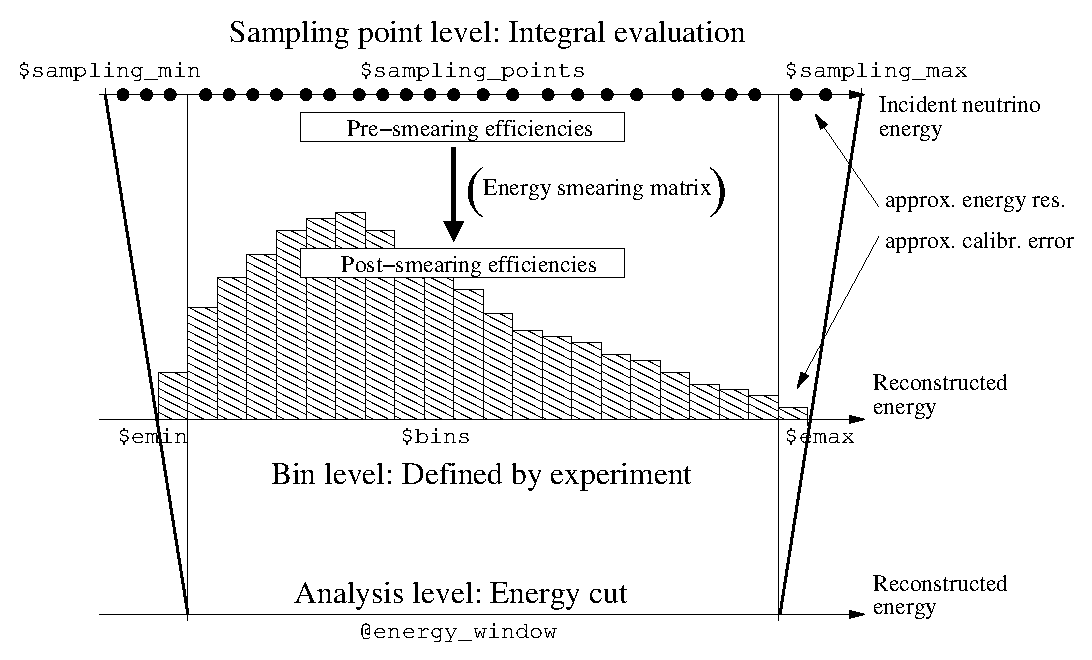
\includegraphics[width=15cm]{energies}
\end{center}
\caption{\label{fig:energies} The different evaluation levels for the energy smearing in \GLOBES .}
\end{figure}

Before we come to the calculation algorithms, it is useful to understand
the general evaluation algorithm. As it is illustrated in \figu{energies}, 
\GLOBES\ uses several levels with respect to the energy ranges:
\begin{description}
\item[Sampling point level]
 This level is used internally to evaluate the integrand in \eq~(\ref{eq:simple_int}) at all sampling points. The energy scale is the actual incident neutrino energy $E$. Note that the sampling range should exceed the energy bin range by about the energy resolution error, since the corresponding sampling points have to be evaluated by the algorithm. 
However, this exceeding is only
necessary to avoid aliasing effects, if the integrand in \eq~(\ref{eq:simple_int}) is large at the limits of the sampling range.
For a manual definition of the sampling points (depends on algorithm), use
\begin{quote}
{\tt
\$sampling\_points = 20\\
\$sampling\_min =          4.0\\
\$sampling\_max =         50.0
}
\end{quote}
for equidistant sampling points. Arbitrarily spaced sampling points can 
be specified analogously to the energy bins below. 
Note that the algorithm expects to 
have at least as many sampling points as energy bins, since otherwise 
the number of (unphysical) sampling constrains the experiment performance.
\item[Bin level] This level is determined by the experiment. Note than energy
bin sizes much smaller than the energy resolution will not improve the results. The energy bin range and the number of energy bins do always have to be specified. For the case of large values of the integrand in \eq~(\ref{eq:simple_int}) at the energy range limits, it is recommended to exceed the analysis energy window by about the energy calibration error in order to avoid aliasing effects.

In order to define a range between $E_\mathrm{min}$
and $E_\mathrm{max}$ divided by a certain number of equidistant bins,
use
\begin{quote}
{\tt
\$emin = 4.0\\
\$emax = 50.0\\
\$bins = 20
}
\end{quote}
For arbitrary bins, use $E_\mathrm{min}$
and $E_\mathrm{max}$ and the size of each bin  $\Delta E_i$:
\begin{quote}
{\tt
\$emin = 4.0\\
\$emax = 50.0\\
\$binsize = \{  15.0 , 5.0 , 20.0, 6.0 \} 
}
\end{quote}
The number of bins will be automatically computed by \GLOBES . Note that the
bin sizes have to add up to the energy range {\tt \$emax}-{\tt \$emin}.
\item[Analysis level]
On the analysis level, an energy window can be defined within each rule. For
details, see next chapter.
\end{description}
In general, the energy smearing happens between the sampling point and bin levels, which means that the energy smearing matrix will have {\tt \$sampling\_points} columns and {\tt \$bins} rows. 

As illustrated in the figure, an interesting feature in combination with the
channels are pre- and post-smearing effects. Pre-smearing effects are taken into account on the sampling point level, and post-smearing effects on the bin level. Examples for these effects are energy 
dependent efficiencies and (non-beam) backgrounds. Efficiencies are multiplicative factors, whereas backgrounds are added to the event rates. These components can be introduced before or after the integration in \eq~(\ref{eq:simple_int}) is done. If they are introduced before, 
we call them
{\tt @pre\_smearing\_efficiencies} or {\tt @pre\_smearing\_background}. 
If they are introduced after, we call them {\tt @post\_smearing\_efficiencies} or {\tt @post\_smearing\_background}.
Note that pre-smearing components are always a function of the incident neutrino energy $E$. Thus, there have to be as  many elements as there are sampling points. For some algorithms, the number of sampling points is determined automatically by \GLOBES , and the number of elements in the  pre-smearing vectors has to be adjusted in the second run.
Examples for pre-smearing quantities are non-beam backgrounds, such as from geophysical neutrinos. The post-smearing components are always a function of the reconstructed neutrino energy $E'$, such as the post-smearing efficiencies $\epsilon_\beta^{\text{IT}}(E')$ in \eq~(\ref{eq:e_res}). Examples for post-smearing efficiencies are cuts and detection threshold functions. All post-smearing components have to have as 
many elements as there are energy bins. Efficiencies are multiplicative 
and their default value is $1$, whereas backgrounds are additive and their default value is $0$. Thus, a more elaborate channel can be defined as
\begin{quote}
{\tt channel(\#channel\_1)<\\
\tb @channel = \#flux : $+$: muon: muon: \#cross: \#energy\\
\tb @pre\_smearing\_background = \{1,2,3,4,5,6,7,8,9,10\}\\
\tb @post\_smearing\_efficiencies = \{0.1,0.2,0.3,0.4,0.5\}\\
>}
\end{quote}
This experiment uses $10$ sampling points and $5$ bins.

In the following subsections we will define the energy resolution function.
All energy resolution functions are defined within an {\tt energy} environment and can be refered to by {\tt \#name}.
\begin{quote}
  {\tt energy(\#name)<\\
\tb $\ldots$\\
>}
\end{quote}
The individual parameters of the environment will be defined below and depend on the algorithm used.

\subsection{Bin-based automatic energy smearing}

This algorithm is the simplest of the built-in algorithms for the evaluation
of \eq~(\ref{eq:simple_int}). It is applicable to most of the
 accelerator-based experiments which can be simulated with \GLOBES .

The key idea is to use a ``flat'' model with sampling points identical to 
the bins (\cf, \figu{energies}). This is a good approximation as long as
\begin{itemize}
\item
 The number of bins is larger than the energy resolution.
\item
 The integrand in \eq~(\ref{eq:simple_int}) is small at the bin range limits
{\tt \$emin} and {\tt \$emax} (in order to avoid aliasing effects).
\item
 The neutrino oscillations are slow on a scale of the bin distance.
\end{itemize}
In this case, \eq~(\ref{eq:simple_int}) is reduced to
\begin{equation}
\label{eq:algo_one}
n_i^c=N/L^2 \, \sum_{j=1}^N \,  \Phi^c(E_j)\,
P^c(E_j)\,
\sigma^c(E_j)\,
K_i^c(E_j) \, \Delta E_j \,.
\end{equation}
The advantages of this algorithm are obvious: All factors
independent of the oscillation parameters have to be only evaluated once
at values of $E$ which are known in advance, which means that they can be put 
into a look-up table. In addition, the probability
has to be only evaluated at previously known values of the energy, which
makes it possible to compute the transition amplitudes for all channels
simultaneously. One assumption is that all involved factors are piece-wise
constant, \ie, they hardly change within each bin. This 
assumption seems to be very restrictive. Note, however, if one analyzes simulated data (which are simulated with the same algorithm), the errors
will cancel between the simulated and fitted data. 
%
Furthermore, we will demonstrate in the next subsection that the assumption
is rather good. ??? COMES THERE ???
%
This algorithm is the fastest which \GLOBES\ offers, and is selected by
\begin{quote}
{\tt \tb @type = 1}
\end{quote}
within the {\tt \#energy} environment.
The computation of the bin kernel $K_i^c$ is performed
by \GLOBES. Thus, it requires  the number of bins
 $N_\mathrm{bins}$
and the minimum $E_\mathrm{min}$ and maximum energy $E_\mathrm{max}$
for equidistant bins.
 
As far as the parameterization for the energy resolution function 
$R^c(E,E')$ in \eq~(\ref{eq:kernel}) is concerned, the algorithm uses
the Gaussian
\begin{equation}
R^c(E,E')=\frac{1}{\sigma(E)\,\sqrt{2\pi}}\,e^{-\frac{(E-E')^2}{2\sigma^2(E)}} \, .
\end{equation} 
CHECK FACTOR OF TWO IN DENOMINATOR WITH SOFTWARE (IMPORTANT)!!! (NORMALIZATION IS OK!)
There are several energy resolution functions available, where by default
{\tt \#standard} is used:
\begin{quote}
{\tt \tb @sigma\_function = \#standard} 
\end{quote}
The energy resolution function {\tt \#standard} is defined by
\begin{equation}
\label{eq:sigma_e}
\sigma(E)=\alpha\cdot E + \beta \cdot \sqrt{E} +\gamma\, ,
\end{equation}
where the parameters $\alpha, \beta$ and $\gamma$ are provided by the user:
\begin{quote}
{\tt \tb @sigma\_e = \{0.15, 0.0, 0.0\}}
\end{quote}
Currently, another possible choice for {\tt @sigma\_function} is {\tt \#inverse\_beta},
which only uses the parameter $\alpha$. It is defined by
\begin{equation}
\sigma(E)= \left\{\begin{array}{cl}
 \alpha \cdot \sqrt{1000}^{-1}\,\sqrt{x-8\cdot10^{-4}}\,,&\mathrm{for}\,\, 
x>1.8\cdot10^{-3}\\
5\cdot10^{-5} \,,&\mathrm{for}\,\, x \leq 1.8\cdot10^{-3}
\end{array} \right.
\end{equation}
In the actual implementation of the algorithm,  the sum in \eq~(\ref{eq:algo_one}) is only computed for the $E_j$'s where $K(E_j)$ 
is above a certain threshold, which is by default $10^{-7}$. 
This threshold is defined at the compiling time. 

Eventually,  a complete energy resolution definition of this 
algorithm is, for example,
\begin{quote}
{\tt energy(\#name)<\\
\tb @type = 1\\
\tb @sigma\_function = \#standard\\
\tb @sigma\_e = \{0.15 ,0.0 ,0.0\}\\
>
}
\end{quote}

\subsection{Low-pass filter based automatic energy smearing}

THIS SUBSECTION WILL BE RE-WRITTEN BY PATRICK (WW)

The second available algorithm is more complicated, a little slower but
much more accurate and much less susceptible to aliasing effects
\index{Aliasing}. The starting
point again is equation~\ref{eq:simple_int}. The idea now is to
 have a good approximation to the integral but still keeping the fixed sampling
point in $E$. To this end we rewrite the integrand of 
equation~\ref{eq:simple_int} using the sampling theorem~\cite{NRC,Rybicki}
\begin{equation}
\label{eq:sampling}
f(E)=\sum_{k=-\infty}^{\infty}\,f(E_k) 
\times \mathrm{sinc}\left(\frac{\pi}{h}(E-E_k)\right)+e(E)
\end{equation}
with $\mathrm{sinc}(x):=\sin(x)/x$ and $E_k=E^0+h\cdot k$. 
This the so called sampling 
representation of the integrand $f(E)$ and $e(E)$ is an error term.
The error term vanishes if the Fourier transform $\hat f(\omega)$ of $f(E)$
is zero outside the interval $[-\pi/h,\pi/h]$. Thus one suspects that
the error term is small once the power beyond $\pi/h$ is low. Furthermore
the sum in equation~\ref{eq:sampling} can be truncated to a few terms if
$f(E)$ has a compact support, \ie\ it is different from zero only 
on a finite interval. Thus the sampling representation is most useful
for functions which have both a compact support in real \emph{and} Fourier
space. This of course is impossible, however the function which comes
most closely to this, is well known -- it is a Gau\ss ian. Our $f(E)$ is not
exactly a Gau\ss ian  but the convolution of a top hat and a Gau\ss ian, thus
its real and Fourier space components still behave rather Gau\ss ian 
especially for large values of $E$ and $\omega$ respectively. The advantage of
using the sampling representation is that the integration with respect to $E$
is easily performed analytically
  \begin{eqnarray}
\label{eq:int_sampling}
\int dE \quad f(E)&\simeq& \sum_{k=k_{l}}^{k_{u}}\,f(E_k) 
\times \mathrm{Si}\left(\frac{\pi}{h}(E-E_k)\right)\,,\\
\mathrm{Si}(x)&:=&\int_{0}^x dx'\quad \sin(x')/x'\,,\nonumber 
\end{eqnarray}
where $k_l$ and $k_u$ are suitable chosen bounds for the summation.

In order to have a good compromise between speed an accuracy the choice
of $h$, $k_l$ and $k_u$ is crucial. The choice of $h$ is governed by the
need to sample $f(E)$ at a sufficient rate in order not to produce aliasing.
For this purpose it useful to consider some properties of the power spectrum
of $f(E)$. Provided the cross section and flux is smooth enough  the only
high power components in $\hat f(\omega)$ are due to a fast oscillating
$P(E)$. We can estimate the largest frequency $\omega_m$ quite easily, it is
given by the largest $\Delta m^2_m$ and the lowest energy $E_l$
\begin{equation}
\omega_m \simeq \frac{\Delta m^2_m \cdot L}{E_l^2}
\end{equation}
On the other hand the finite energy resolution of any real detector anyhow
will act as a low-pass filter eliminating any power beyond $\sim 1/\sigma(E)$.
For now we assume that there are no frequencies which are not resolved by
the detector thus the sampling frequency is determined by the energy 
resolution of the detector. In that case the correct sampling 
width $h$ is approximately
\begin{equation}
h\simeq 1/\sigma(E_l)\,.
\end{equation} 

The range for the summation $k_l^i$ and $k_u^i$ is given by the range of 
integration $a_i$ and $b_i$ in equation~\ref{eq:simple_int}, the integration 
limits there are $0$ to $\infty$. For practical purposes however the range
can be reduced to $a_i$ and $b_i$. They are  determined by requiring
that the area under the bin kernel $K_i^c$ has reached a specific 
value close to one,
the so called confidence level $c$ (new name would be better). $1-c$ is a 
small number and specifies the fraction of  events in bin which lie outside
the summation range, usually $1-c=10^{-3}$ is sufficient. Furthermore the
value of the bin kernel at the lower and upper boundary should
be the same
\begin{eqnarray}
\int_{a_i}^{b_i} dE\quad K_i^c(E) &=& c\,,\\
K_i^c(a_i)&=&K_i^c(b_i)\,.
\end{eqnarray} 
Knowing $a_i$ and $b_i$ it is easy to obtain $k_l$ and $k_u$ by requiring
that the summation extends one bin beyond  each $a_i$ and $b_i$. Furthermore
it is possible to specify an offset which extends the index range on each side
by its value.

Since the $a_i$'s and $b_i$'s are not known in advance it could be possible
that $a_0$ and/or $b_{N_\mathrm{bins}}$ lie outside the computational domain,
\eg\ no cross section or flux is defined at those energies. To remedy this 
problem the computational domain can be specified. No calculation in \GLOBES\
will leave this domain. 

In order to ensure that fast oscillating probabilities do not lead to aliasing
it is desirable to impose a low-pass filter already during the calculation
of the probabilities itself. This is possible and implemented has a highly
experimental feature called ``filter''\index{Filter}. 
The calculation of oscillation
probabilities basically is a computation of phase differences. Restricting
the maximum admissible size of those phase difference effectively filters
the high frequency component of the oscillation probability. This idea is
implemented according to
\begin{eqnarray}
\label{eq:filter_a}
P_{\alpha\beta}(E)&=&\sum_{ij}
U_{\alpha j} U^*_{\beta j} U^*_{\alpha i} U_{\beta i} 
e^{-i\Phi_{ij}}\times 
e^{ -\Phi_{ij}^2/\sigma_f(E)^2 }\,,
\end{eqnarray}
where $\Phi_{ij}:=\Delta m_{ij}^2 L/2E$ is the usual phase difference and
the last term is a Gau\ss ian filter with width $\sigma_f(E)$. Choosing
$\sigma_f(E):=\sigma_f^0 \cdot E$ ensures that this filter behaves 
approximately like an energy resolution function with constant width 
$\sigma_e=\sqrt{2}/\sigma_f^0$, \ie\
\begin{equation}
\label{eq:filter_b}
\int d\tilde E\quad P(\tilde E) \frac{1}{\sigma_e\,\sqrt{2\pi}}\,
e^{-\frac{(E-\tilde E)^2}{2\sigma^2_e}}\,.
\end{equation}
The equivalence of equation~\ref{eq:filter_a} and equation~\ref{eq:filter_b}
is not obvious and connected to the properties of $P_{\alpha\beta}$, 
see~\cite{Kiers:1996zj,Giunti:2003ax}. This feature works \emph{only} 
for vacuum and constant densities and controlled
by the filer state variable and $\sigma_f^0$ is set by the filter value 
variable. Assuming that $P_{\alpha\beta}$ still is the source for the highest
frequencies one can split the energy resolution function $\sigma(E)^c$ in
two parts by
\begin{equation}
\sigma_c^2(E)=\underbrace{\sigma_c^2(E)-\sigma_c^2(E_\mathrm{min})}_
{\tilde\sigma^2_c(E)}+\underbrace{\sigma_c^2(E_\mathrm{min})}_{\sigma_e^2}\,,
\end{equation}
where $\tilde\sigma_c(E)$ is used instead of $\sigma_c(E)$ in computing the
smearing data and $\sigma_e$ is used to determine $\sigma_f^0$.

\subsection{Manual energy smearing}

In some cases, one may use the output of a detector Monte Carlo simulation
directly. Then one can use manual energy smearing instead of one of the
automatic energy smearing algorithms. 

The energy smearing matrix $K_{ij}$ has {\tt \$bins} rows and {\tt \$sampling\_points} columns, which are numbered from $0$ to {\tt \$bins}$-1$ or {\tt \$sampling\_points}$-1$. It is equivalent to the 
bin- and sampling-point-based kernel in \eq~(\ref{eq:kernel}):
\begin{equation}
K_{ij} = K_i^c(E) |_{E=E_j},
\label{equ:ematrix}
\end{equation}
where $E_j$ is the energy of the $j$th sampling point. In general, many of the entries in this matrix are zero, which means that it is convenient to evaluate the integrand in \eq~(\ref{eq:simple_int}) only at positions where
$K_{ij}$ is non-zero. The corresponding ``sampling range'' range of non-zero matrix entries  in $K_{ij}$ for the $i$th energy bin is defined to run from
column $k_l^i$ (``lower index'') to column $k_u^i$ (``upper index'').
An example for a smearing matrix is
\begin{equation}
K_{ij} =   \underbrace{ \left( \begin{array}{cccccccccc} 
a_{00} & a_{01} & a_{02} & a_{03} &  &  &  &  &  & \\
a_{10} & a_{11} & a_{12} & a_{13} & a_{14} &  &  &  &  &  \\
 & a_{21} & a_{22} & a_{23} & a_{24} & a_{25} &  &  &  &  \\
 &  & a_{32} & a_{33} & a_{34} & a_{35} & a_{36} &  &  &  \\
 &  &  & a_{43} & a_{44} & a_{45} & a_{46} & a_{47} &  &  \\
& & & \uparrow  & & \ddots & & \uparrow & & \\
& & & k_l^i & & & & k_u^i & & \\ 
\end{array}\right) }_{\mathtt{\$sampling\_points}  \, \, \mathrm{columns}} \quad \leftarrow \quad \footnotesize{\mathtt{\$bins} \, \, \mathrm{rows}} \, ,
\end{equation}
where the unshown entries are zero. Thus, the values of $K_{ij}$ have to be specified between $k_l^i$ and $k_u^i$ in the form $\{ k_l^i,k_u^i, K_{i \, k_l^i}, K_{i k_l^i+1} , \hdots , K_{i k_u^i} \}$:
\begin{quote}
{\tt 
energy(\#name)<\\
\tb @energy =   \{0,2, 0.8634265, 0.0682827,     4e-06\}:\\
\tb\tb \{0,4, 0.1507103, 0.6965592, 0.1507103,   0.00101,     1e-07\}:\\
\tb\tb $\ldots$\\
>
}
\end{quote}
Note that the sum of all entries in each {\em column} should be equal 
to unity,
since all of the incoming neutrinos should be assigned to energy bins. In many practical cases, however, the definition of the energy smearing can
lead to sums smaller than unity, such as in the case of truncated Gaussian
distributions. The sum of entries in each {\em row} is not defined, since the events might be unevently distributed into the energy bins
according to the energy resolution function.

%%%%%%%%%%%%%%%%%%%%%%%%%%%%%%%%%%%%%%%%%%%%%%%%%%%%%%%%%%%%%%%%%%%%%%%%%%%%
\section{Rules and the treatment of systematics}
\label{sec:rules}

The set of rules\index{Rule} for an experiment is the final 
link between the event rate computation and the statistical analysis. 
The information in the rules
specifies how the $\chi^2$ is computed based upon the raw event rates 
given by the channels and possible systematical errors. 
Therefore a rule has two parts: The first part describes how signal and 
background events are composed out of the channels, and the second part
specifies which systematical errors are considered, as well as their values.
%
For a rule, the splitting
in signal and background is useful for simplicity and the treatment of systematics, as we will se later. Each rule will lead to a $\chi^2$-value,
which means that all $\chi^2$'s of the different rules will be added
for the whole experiment. Within each rule, the event rates are added, and
the systematics is considered to be independent of the other rules.
Thus, it is convenient to combine the above defined channels for different
oscillation patterns and interaction types into one logical construction,
which is the rule. For example, a superbeam usually has two rules: One for
the $\nu_e$-appearance rates, and one for the $\nu_\mu$-disappearance rates.
 In each case, contributions of several interaction types, as well as from
 the $\nu_e$-contamination of the beam will lead to a number of contributing signal and background event channels.


% WEITER:

Based on the definition of channels it is possible to assemble the 
signal and background event numbers for each bin.  
The signal $s_i$ in one bin for a rule now can be composed out of 
several channels by (OFTEN ONLY ONE) 
\begin{equation}
s_i=\epsilon_{c_1}\cdot n_i^{c_1}\,+\,\epsilon_{c_2}\cdot n_i^{c_2}\,+\,\ldots
\end{equation}
where the $\epsilon$'s are weight factors determined by the properties
of the detector.
Similarly the background in one bin $i$ can be specified by
\begin{equation}
b_i=\epsilon_{c_1}\cdot n_i^{c_1}\,+\,\epsilon_{c_2}\cdot n_i^{c_2}\,+\,\ldots
\end{equation}
This basic building blocks of a rule are specified by
\begin{quote}
{\tt \tb @signal = 0.5 @ \#channel\_1\\
\tb @background = 0.001 @ \#channel\_2 :  0.005 @ \#channel\_3
}
\end{quote}

Quite often it is not sufficient to have constant efficiencies and therefore
it is possible to define efficiencies for each bin and channel $\alpha_i^c$
and thus the event rates in one bin become
\begin{equation}
s_i=\epsilon_{c_1}\alpha_i^{c_1}\cdot n_i^{c_1}\,+
\,\epsilon_{c_2}\alpha_i^{c_2}\cdot n_i^{c_2}\,+\,\ldots\,,
\end{equation}
and analogous for $b_i$.



The set of all $s_i$'s and $b_i$'s now can be composed in a form that takes
some types of systematical error into account. The two most important and
most easily parameterized systematics are a normalization and an energy
calibration error. These error are considered separately for the signal events
and the background events. The implementation of the normalization error
is straight forward
\begin{equation}
s_i(a):=a\cdot s_i
\end{equation} 
with an analogous definition for the background events.

For the parameterization of an energy calibration error two possibilities
are implemented. The first one being somewhat simpler, whereas the second one
is more accurate but requires a careful choice of parameters. The first 
option is
\begin{equation}
s_i(a,b):=s_i(a)+b\cdot s_i\, E_i/(E_\mathrm{max}-E_\mathrm{min})
\end{equation}
and it is refered to as tilt since it describes a linear distortion, a tilt
of the event rate spectrum. The second option is closer to an actual energy
calibration error, which basically amounts to replacing the reconstructed 
energy $E'$ by $(1+b)\cdot E'$ and we use following approximation
\begin{eqnarray}
s_i(b)&=& (1+b)\cdot(s_{k+1}-s_k)\cdot\delta+s_i\,,\\
\delta&=&b\cdot(i+t_0+ 1/2)+i\,,\nonumber\\
k&=&\mod(\delta,1)\,,\nonumber\\
t_0&=&E_\mathrm{min}/\Delta E_0\,.\nonumber
\end{eqnarray}
Special care is required at the boundaries when $k<1$ or $k+1>N_\mathrm{bins}$,
since there $s_k$ or $s_{k+1}$ may not have been calculated. One possibility
to deal with those cases is to assume that for those values of $k$ $s_k$ is
zero. This is the default. In cases where $s$ at the boundary is however still
sizeable this may lead to intolerable errors and subsequently to a wrong
estimate of the impact of a calibration error. Therefore in those cases it
is advisable to truncate the analysis range by a few bins at the boundary
and therefore ensure in this way that only those $s_i$ are used whose index
$k$ is within the range $1,\ldots, N_\mathrm{bins}-1$. 

In order to perform this fine tuning, it is possible to constrain 
the energy range from which the data are taken for the 
analysis\index{Energy window}. This is achieved by setting the energy window
variable. 
\begin{quote}
{\tt 
\tb @energy\_window = 4.0 : 50.0 
}
\end{quote}
The purpose is mainly to allow a fine tuning of the description
of an energy calibration error. The default setting is that the energy window
coincides with the range defined by the minimal and maximal reconstructed 
energy. For the error dimension using the calibration method (C) it is 
advisable to reduce the energy window by two or three bins at both the lower
and upper end. As a rule of
thumb consider the three standard deviations error on the calibration and
evaluate the corresponding shift in $E'$ at the lower and upper energy limit 
and reduce the analysis range by this amount.

Thus the total event rate $x_i$ in a bin $i$ is given by
\begin{equation}
x_i(a,b,c,d)=s_i(a,b)+b_i(c,d)
\end{equation}
and thus a function of four parameters. The central values for all of
the four parameters are always needed. They are called signal normalization
($a$), signal tilt/calibration ($b$), background  normalization ($c$) and
background tilt/calibration ($d$). The default values are
\begin{equation}
a=1\,,\quad b=0\,,\quad c={\tt NaN}\,,\quad d=0\,,
\end{equation}
thus for the background normalization $c$ a value has to be specified in 
\emph{all} cases. The central values for the normalization and the 
corresponding central value of tilt/calibration are regarded
as a pair. The errors are treated in the same way.
\begin{quote}
{\tt
\tb @signalerror =       0.001  :       0.01\\
\tb @backgroundcenter =  0.1 :       0.0\\
\tb @backgrounderror =   0.001 :       0.01
}
\end{quote}
There is no {\tt @signalcenter} since by default the central value for the
signal normalization is $1$ and the central value for the tilt/calibration 
is $0$.  

The four parameters $a,b,c,d$ have been introduced in order to describe
systematical uncertainties, they are so called nuisance parameters.
For the analysis of the systematical errors the so called 
 pull method is 
used~\cite{Fogli:2002pt}\footnote{In fact the pull method
was employed already in~\cite{Huber:2002mx} before 
\cite{Fogli:2002pt} appeared.}. 
In the  pull method $k$ systematical errors are included by introducing 
$k$ additional variables $\zeta_k$, which will  be called 
nuisance parameters in the following. 
The nuisance parameters describe the dependence of the event rates on the 
various sources of systematical errors, \eg\ an error on the total 
normalization is included by multiplying the expected number of events in 
each bin by a factor $(1+\zeta_1)$. The variation of $\zeta_1$ in the fit 
is constrained by adding a penalty $p_1$ to the $\chi^2$-function. In case 
of a  Gau\ss ian distributed systematical error this penalty is 
given by
\begin{equation}
\label{eq:penalty}
p_i=\frac{(\zeta_i-\zeta_i^0)^2}{\sigma_{\zeta_i}^2}\,,
\end{equation}
where $\zeta_i^0$ denotes the mean and $\sigma_{\zeta_i}$ the standard 
deviation of the corresponding nuisance parameter, \ie\ the amount of 
systematical uncertainty. 
The resulting $\chi^2$ is then minimized with respect to all nuisance 
parameters $\zeta_i$ and this yields $\chi^2_\mathrm{pull}$
\begin{equation}
\chi^2_\mathrm{pull}(\boldsymbol{\lambda}):=\min_{\{\zeta_i\} } \,\, \left( 
\chi^2(\boldsymbol{\lambda},
\zeta_1, \ldots, \zeta_k)+ \sum_{j=1}^{k} p_j(\zeta_j)\right)\,,
\end{equation}
where $\boldsymbol{\lambda}$ denotes the oscillation parameters 
including the matter density
$\rho$. One advantage of the pull method is that whenever the number $N$ of 
data points is much larger than $k$, it is numerically easier to compute 
$\chi^2_\mathrm{pull}$ than to invert the $N\times N$ covariance matrix. For
the experiments considered here $N$ is typically $20$ and $k\sim 4$, thus
the pull method is numerically much faster. Moreover it is more flexible and 
allows the inclusion of systematical errors also for a 
Poissonian $\chi^2$-function.
In~\cite{Fogli:2002pt} it was shown that the pull method and the covariance
based approach are equivalent for a Gau\ss ian and linear model. In general
there is a separate $(\chi^2_\mathrm{pull})^\alpha$ for each rule $\alpha$, 
\ie\ pair of signal and background spectra, with a separate set of 
nuisance parameters $\zeta_i^\alpha$. In this case $\chi^2_\mathrm{pull}$
is the sum of all individual  $(\chi^2_\mathrm{pull})^\alpha$.
In this way the dependence on the $k$ nuisance parameters has been eliminated 
from $\chi^2_\mathrm{pull}$. 

The user has the possibility to choose the set $\{\zeta_i\}$ of nuisance 
parameters which are marginalized. This achieved with the error dimension 
variable\index{Error dimension}, and the different possibilities are shown in
table~\ref{tab:error_dim}. If a parameter is designated with $+$, it will
be marginalized and therefore the corresponding error needs to have a non-zero
value. In the cases labeled (number 4 and 8) ``total rates'' 
the summation over the bins is performed \emph{before} computing 
the $\chi^2$. The case labeled (number 7) ``spectrum only'' leaves the 
normalization free ($\sigma_a=\sigma_c=\infty$) and therefore counts only the 
spectral information in the data. As a consequence
the settings for the normalization error will be ignored. It is furthermore
possible to extend the set of error dimensions and thus the set of possible 
systematical errors to be studied, but this requires proper C programing, 
compiling and linking with \GLOBES. The interface for user defined error 
dimensions is described in detail in section~\ref{sec:ud_error_dim}.

%%%%%%%%%%%%%%%%%%%%%%%%%%%%%%%%%%%%%%%%%%%%%%%%%%%%%%%%%%%
\begin{center}
\begin{table}[hbt!]
\begin{center}
\begin{tabular}[h]{|c|cccc|c|c|}
\hline
Error dimension&$a$&$b$&$c$&$d$&Tilt/Calibration&Remarks\\
\hline
\hline
0&+&+&+&+&T&\\
2&-&-&-&-&-&\\
4&+&+&+&+&T&total rates\\
7&o&-&o&-&-&spectrum only\\
8&-&-&-&-&-&total rates\\
9&+&+&+&+&C&\\
\hline
\end{tabular}
\caption[Table of error dimensions]{\label{tab:error_dim}
Values of the error dimension variable and their meaning.
 }
\end{center} 
\end{table} 
\end{center}
%%%%%%%%%%%%%%%%%%%%%%%%%%%%%%%%%%%%%%%%%%%%%%%%%%%%%%%%%%%%%%

The error dimensions can be chosen for each rule by
\begin{quote}
{\tt 
\tb @errordim = 1
}
\end{quote}

Next we can assemble the various pieces into one rule
\begin{quote}
{\tt rule(\#rule\_1)<\\
\tb @signal = 0.5 @ \#channel\_1\\
\tb @background = 0.001 @ \#channel\_2 :  0.005 @ \#channel\_3\\
\tb @signalerror =       0.001  :       0.01\\
\tb @backgroundcenter =  0.1 :       0.0\\
\tb @backgrounderror =   0.001 :       0.01\\
\tb @errordim = 1\\
\tb @energy\_window = 4.0 : 50.0\\ 
>}
\end{quote}


%%%%%%%%%%%%%%%%%%%%%%%%%%%%%%%%%%%%%%%%%%%%%%%%%%%%%%%%%%%%%%%%%%%%%%%%%%
%\section{User-defined systematics}
%\label{sec:ud_error_dim}.


%%% Local Variables: 
%%% mode: latex
%%% TeX-master: Manual.tex
%%% End: 
